\chapter{Tanulásmenedzsment rendszerek IT infrastruktúrája}

Ebben a fejezetben a háromrétegű architektúra példáján alapulva részletezem az oktatástámogató rendszerek IT infrastruktúráját, majd egy megvalósítást részletesebben is bemutatok. 

\section{A háromrétegű architektúra}
A webes LSM-ek általában a háromrétegű architektúrát követik. Ez a három réteg a webkiszolgáló, az adatbázis és az alkalmazás réteg. A réteges szerkezetnek köszönhetően ezek a rendszerek jól skálázhatóak, gyakran az egyes rétegekben a réteget megvalósító alkalmazások olyan tulajdonságokkal, funkciókkal rendelkeznek, amelyek támogatják is a skálázás egyszerű, esetleg automatikus megvalósítását.

\begin{figure}[!ht]
\centering
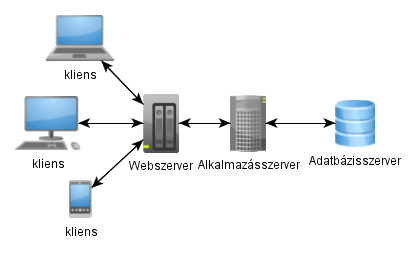
\includegraphics[width=100mm, keepaspectratio]{figures/3tier_simple_001.png}
\caption{A háromrétegű architektúra.}
\label{fig:3tier_simple_001}
\end{figure}

\Aref{fig:3tier_simple_001}.~ábrán látható elrendezéssel ellentétben a rétegeknek nem szükséges fizikailag is külön hardverre kerülni (sőt az alkalmazás- és webkiszolgáló-réteg esetében ez nem is mindig lehetséges), így a legegyszerűbb kialakítás akár egy számítógépet is igénybe vehet. Ez a megoldás egy viszonylag erős konfiguráció és alacsony felhasználószám esetén működhet.

\subsection{A webkiszolgáló réteg}
A webkiszolgáló réteg feladatát egy szolgáltatás látja el, amely futhat egy vagy több példányban, és egy példány futhat egy vagy több számítógépen is. Ez a szolgáltatás felelős azért, hogy a kliensek kérésének megfelelően előálljon a weblap, vagyis a kliensek kérésre kapjanak egy HTML dokumentumot, amelyet a felhasználói oldalon jelenítenek meg.
A piacon több webkiszolgáló alkalmazást találunk, ezek közül van ingyenes, nyílt forráskódú (pl. Apache), és kereskedelmi termék is (Microsoft IIS).

\Aref{fig:netcraft_webservers}.~ábrán a legelterjedtebb webkiszolgálók piaci részesedésének alakulása látható.

\begin{figure}[h!]
\centering
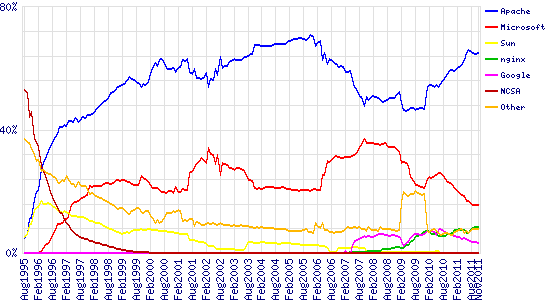
\includegraphics[width=1.0\textwidth]{figures/wpid-overallc.png}
\caption{A legelterjedtebb webszerverek piaci részesedése (2011. november, forrás: \href{http://news.netcraft.com/archives/2011/11/07/november-2011-web-server-survey.html}{Netcraft.com}) \label{fig:netcraft_webservers}}
\end{figure}

Az oktatástámogató rendszerek szempontjából fontos, hogy a működtetett webkiszolgáló képes legyen nagy számú konkurens kérés kiszolgálására, vagy könnyen skálázható, elosztható legyen. LMS-ek esetén is ugyanazokat a webkiszolgálókat lehet használni, mint amit más egyéb webes alkalmazások esetén (pl. Apache, Microsoft IIS, lighttpd, ngnix, stb.).
 
\subsection{Az alkalmazás réteg}
Az alkalmazás réteg feladatát az alkalmazásszerver látja el. Az alkalmazásszerver egy olyan speciális környezet, ahol alkalmazások futhatnak, és amely környezet szempontjából lényegtelen, hogy mik ezek az alkalmazások és mit csinálnak\cite{serverside}. Az alkalmazásszerver eljárások (programok, rutinok, szkriptek) hatékony végrehajtására dedikált erőforrás.

Az első alkalmazásszerverek megjelenésekor fő feladatuk volt, hogy webes alkalmazások esetén a webszerver által megjeleníthető tartalmat állítsanak elő. Ezen továbblépve napjainkban már nem csak az oldalgenerálás funkciója jelenik meg ebben a rétegben, hanem egyéb szolgáltatásokat is implementálnak, mint például klaszterszervezést, terheléselosztást, hibaátállást. Ezen funkciókkal elérhető, hogy az alkalmazásfejlesztőknek csak az üzleti logikával kelljen foglalkozni.

Az LMS-ek lényegi része ebben a rétegben kerül megvalósításra. Mivel a ténylegesen alkalmazott platformtól függ, hogy milyen alkalmazásszervert használunk, ezért alapvetően erről az oldalról nincs megkötés. Ám érdemes figyelembe venni, hogy a kiválasztott platform mennyire skálázható, milyen teljesítményt nyújt a különböző terhelésekre. A legelterjedtebb LMS-ek fejlesztésére használt platformok itt is mint más webes rendszereknél a PHP, Java és .Net.

\subsection{Az adatbázisréteg}
Az adatbázisréteg feladatait az adatbázisszerver látja el. Adatbázisszervernek nevezünk egy dedikált szolgáltatást, ami adatbázisokat tesz elérhetővé, kezelhetővé. Valójában egy felületet biztosít az alkalmazásrétegben található adatfelhasználó alkalmazás és maguk a felhasználandó adatok között.

Az LMS-ek oldaláról igény, hogy a használt adatbázis képes legyen nagy számú konkurens tranzakcióra, és optimálisan tároljon nagy, multimédiás adatokat is. Főleg a költségvetéstől és az üzemeltetéstől függően lehet MySQL, PostgreSQL, Microsoft SQL Server vagy Oracle adatbázisszerver is, de természetesen attól is függ, hogy az adott LMS melyiket támogatja. 

\section{Egy példa: a Moodle rendszer}
Az oktatástámogató rendszerek közül a Moodle rendszerrel részletesebben foglalkoztam. A következő részben bemutatom az általam megismert felépítését, fontosabb jellemzőit, és ejtek néhány szót az általam telepített rendszerről is.

\subsection{A Moodle rendszer felépítése, tulajdonságai}
Az e-learning rendszerek közül a legelterjedtebb a Moodle (Modular Object-Oriented Dynamic Learning Environment) (\href{http://moodle.org}{http://moodle.org}) nevű tanulásmenedzsment rendszer. Korábbi munkám során ennek a rendszernek a részletesebb megismerése volt az egyik cél.

A Moodle  egy ingyenes és nyílt forrású LMS vagy VLE (Virtual Learning Environment, virtuális oktató környezet). 2010 októberében 49952 regisztrált Moodle oldal létezett, amelyek összesen mintegy 37 millió felhasználót szolgáltak ki. A legnagyobb rendszertelepítések közé tartozik a tajvani Ming Chuan Egyetem több mint 63.000 regisztrált, maximálisan 33.000 bejelentkezett felhasználóval naponta \cite{moodleinstplus}.

Maga a rendszer tervezéséből és implementálásából eredően portábilis, hála a PHP nyelvnek. Módosítás nélkül telepíthető Unix, Linux variánsokra, FreeBSD-re, Windows-ra, Mac OS X-re, NetWare-re és egyéb rendszerekre, amelyek támogatják a PHP-t és az ismertebb adatbázis-kezelő rendszereket.

A Moodle architektúrájában elválik a natív adatbázis-kezelő a felsőbb rétegektől. Közöttük egy ADOdb adatbázis absztrakciós réteg található. Az ADOdb egy különálló projekt\footnote{\href{http://adodb.sourceforge.net/}{http://adodb.sourceforge.net/}}, amely a legelterjedtebb adatbázis-kezelőket támogatja. \Aref{fig:moodlearch}.~ábrán egy korábbi verzió architektúrája látható.

\begin{figure}[h!]
\centering
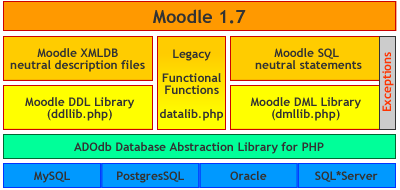
\includegraphics[width=0.65\textwidth]{figures/moodlearch.png}
\caption{A Moodle architektúrája \label{fig:moodlearch}}
\end{figure}

Az architekturális felépítésből látható, hogy a Moodle az ADOdb által nyújtott rétegen keresztül egységesen éri el az eltérő adatbázis-megvalósításokat anélkül, hogy foglalkoznia kellene az ezekből eredő problémákkal.  

Az interoperabilitás több Moodle képességben megjelenik, ilyenek például:
\begin{sajat_itemize}
\setlength{\itemsep}{0pt}
\item autentikáció LDAP-on, Shibboleth-en keresztül
\item kérdések/kérdéssorok importálása/exportálása több formátumban (pl. XML, XHTML stb.)
\item erőforrások kezelése (SCORM, AICC)
\item integráció más tartalomkezelő rendszerekkel (Drupal, Postnuke).
\end{sajat_itemize}

A Moodle fontos tulajdonsága a modularitás, vagyis a rendszer funkcionalitásának könnyű bővíthetősége. Ezt plug-inokkal valósítják meg, amelyek fejlesztését különböző API-k segítik. Ilyen plug-inok pl. a különböző jelentések (reportok), blokkok, portfóliók, tárolók (repository-k), kereső modulok. Ezek közül nagyon sok megtalálható az alap Moodle telepítésben is, de saját magunk is írhatunk hasonló kiegészítőket.

\subsection{Egy lehetséges infrastruktúra kialakítás a Moodle esetében}

Mint azt már említettem, a Moodle nagyon sok operációs rendszerre telepíthető. Én az egyik legelterjedtebb telepítési környezet választottam ki, egy ún. LAMP (Linux - Apache - MySQL - PHP) megoldást használtam. Fizikai szerver helyett virtuális szervert alkalmaztam a Simonyi Károly Szakkollégium Kollégiumi Számítástechnikai Kör erőforrásainak igénybevételével. A virtualizációs megoldás alapja egy VMware ESX szerver volt.
A virtuális szerverem konfigurációja viszonylag gyengének számít, ám nem is volt cél, hogy nagy számú felhasználót szolgáljon ki:
\begin{sajat_itemize}
\item Ubuntu Server 10.10 32bit
\item 512 MB RAM
\item 10 GB tárhely
\item 4 MB RAM a videóvezérlőnek 
\end{sajat_itemize}
Az így kialakított struktúra tulajdonképpen egy egygépes megoldás, mind a webszerver, az alkalmazásszerver, mind az adatbázisszerver egyetlen virtuális gépen futott. Természetesen az infrastruktúra méretét lehetett volna növelni, bonyolítani monitorozó, naplófeldolgozó, biztonsági mentés készítő megoldásokkal, de ez szintén nem volt a feladat része.
